\newcommand{\documenttype}{Bachelor Thesis}
\newcommand{\thesistitle}{A Title to the Report}
\newcommand{\thesissubtitle}{A Catchy Optional Subtitle that Grabs the Attention}

\newcommand{\thesisauthor}{Your Full Name} % Your name :) 
\newcommand{\studentnumber}{090XXXXXX}
\newcommand{\thedate}{Date, year} % For example "June, 2022"

\newcommand{\department}{ITU Physics Engineering}
\newcommand{\departmentdescriber}{Faculty of Science and Letters}
\newcommand{\addressI}{ITU Ayazaga Campus, FEB Building}
\newcommand{\addressII}{34469 Maslak-Istanbul}
\newcommand{\departmentwebsite}{www.itu.edu.tr/en}

% Colours 
\newcommand{\targetcolourmodel}{cmyk} % rgb for a digital version, cmyk for a printed version. Only use lowercase
\selectcolormodel{\targetcolourmodel}

% Define colours from https://www.itu.edu.tr/hakkimizda#kimlik

\definecolor{navyblue}  {rgb/cmyk}{0, 0.267, 0.486 / 1.00, 0.45, 0.00, 0.51}
\definecolor{honeyyellow}  {rgb/cmyk}{0.706, 0.592, 0.349 / 0.00, 0.16, 0.51, 0.29}

\newcommand{\itulogocolour}{white} % Colour of the ITU logo: white, black
\newcommand{\frontpagetextcolour}{white} % front page text colour: white
\colorlet{frontbackcolor}{navyblue} % Set the background colour of the front- and back page.

\begin{titlepage}

\newgeometry{left=11mm,right=11mm,top=50mm,bottom=0pt}
\pagecolor{frontbackcolor}
\color{\frontpagetextcolour}

{ % Thesis title 
\Huge
\begin{tabular}{p{\linewidth}}
\textbf{\thesistitle}  \\ 
\LARGE{\thesissubtitle} \bigskip \\ 
{\huge \documenttype}
\end{tabular}
}

% ITU Department
\begin{tikzpicture}[remember picture,overlay]
\node[anchor=north east, 
      xshift=-10mm, 
      yshift=-12mm] 
      at (current page.north east) 
      {
        \color{\frontpagetextcolour}
        \begin{tabular}{r} 
        \large{\textbf{\thesisauthor}} \\ 
        \studentnumber
        \end{tabular}
      }; 
\end{tikzpicture}

% ITU logo
\begin{tikzpicture}[remember picture,overlay]
\node[anchor=north west, 
      xshift=8.9mm, 
      yshift=-8.3mm] 
     at (current page.north west) 
     {
\includegraphics[width=34.75mm,keepaspectratio]{structure/structure_figures/itu_white_logo.pdf}}; 
\end{tikzpicture}

% Thesis cover photo
\begin{tikzpicture}[remember picture,overlay]
\node[anchor=south, % anchor is bottom of picture
      xshift=0pt, 
      yshift=-2.9mm] % shifting picture to actually be at the bottom of the page
     at (current page.south) % placement at bottom of the page
     {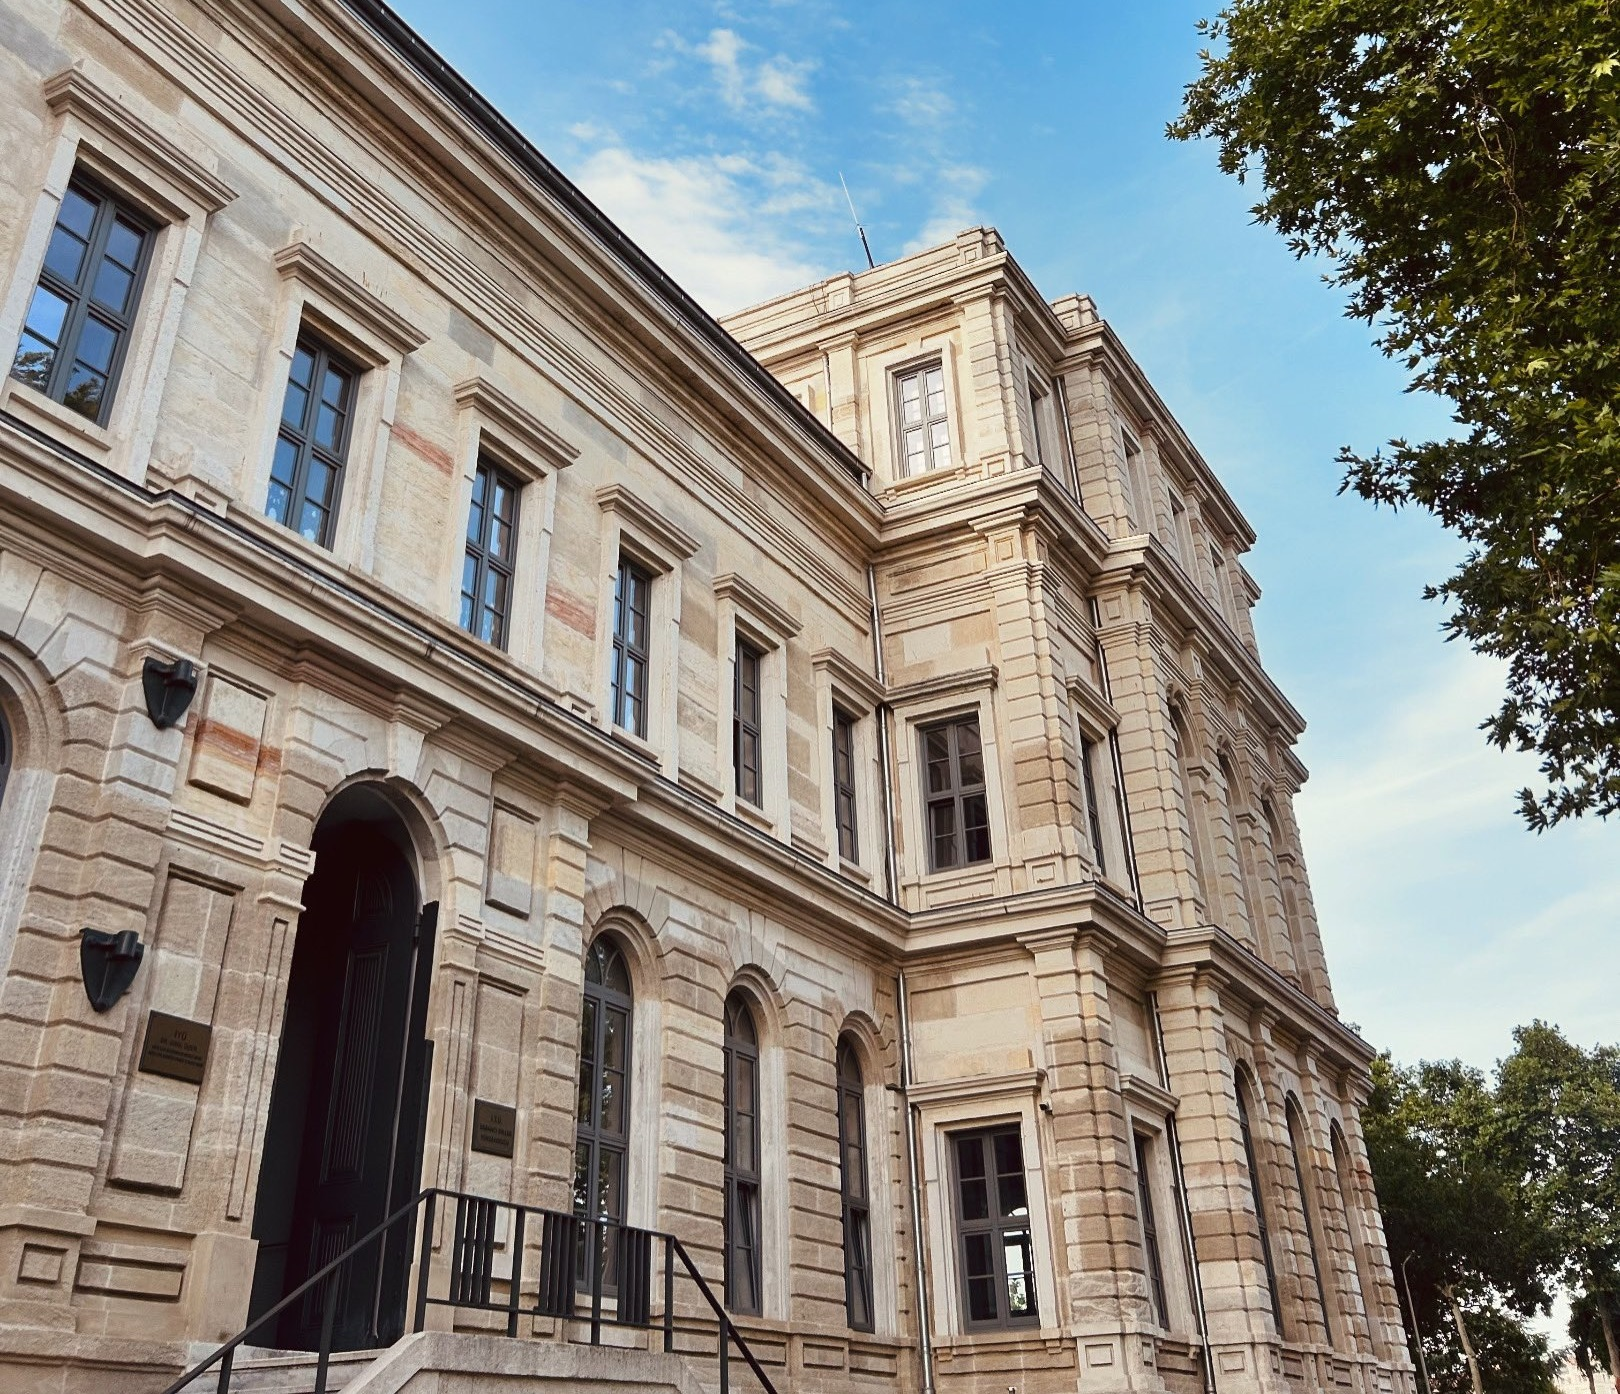
\includegraphics[height=18.9cm,keepaspectratio]{structure/structure_figures/itu_thesis_cover_photo.jpg}};
\end{tikzpicture}




\end{titlepage}